\section{Results}
\label{sec:results}
This section evaluates the key components of our mapping pipeline, beginning with the perception front-end. We first present a quantitative benchmark of various dense depth estimation and semantic segmentation models to assess their performance in the synthetic lunar environment. Subsequently, we analyze the final 3D reconstruction quality, evaluating how the selected perception models impact the geometric accuracy and semantic fidelity of the map. Both quantitative metrics and qualitative results are provided to support the analysis.
The experiments were performed on a system equipped with an Intel i9-14900K CPU (32 cores, 5.7\,GHz), 128\,GB RAM, and an NVIDIA GeForce RTX 4090 GPU with 24\,GB VRAM.
All results related to computational requirements (such as memory usage and runtime) are only indicative, as the current implementation, methods, and models have not been optimized.

\begin{figure*}[b!]
	\centering
	\begin{subfigure}[b]{0.16\textwidth}
		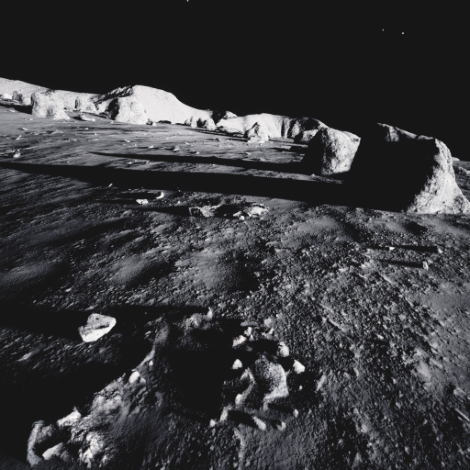
\includegraphics[width=\textwidth]{figures/rgb.png}
		\caption{\bfseries Input}
	\end{subfigure}\hfill
	\begin{subfigure}[b]{0.16\textwidth}
		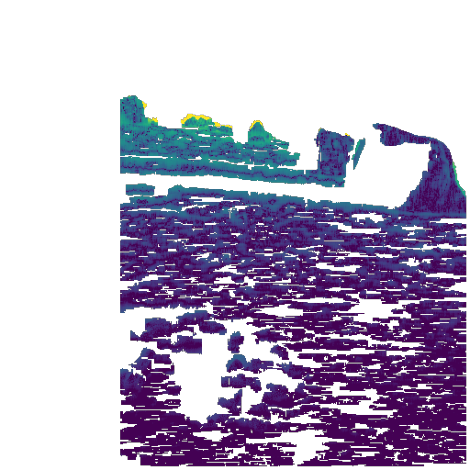
\includegraphics[width=\textwidth]{figures/depth_error_BM.png}
		\caption{\bfseries BM}
	\end{subfigure}\hfill
	\begin{subfigure}[b]{0.16\textwidth}
		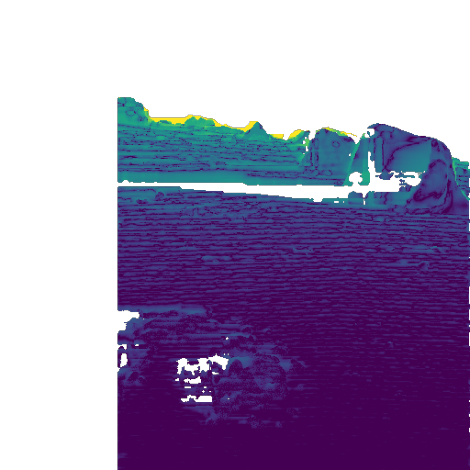
\includegraphics[width=\textwidth]{figures/depth_error_SGBM.png}
		\caption{\bfseries SGBM}
	\end{subfigure}\hfill
	\begin{subfigure}[b]{0.16\textwidth}
		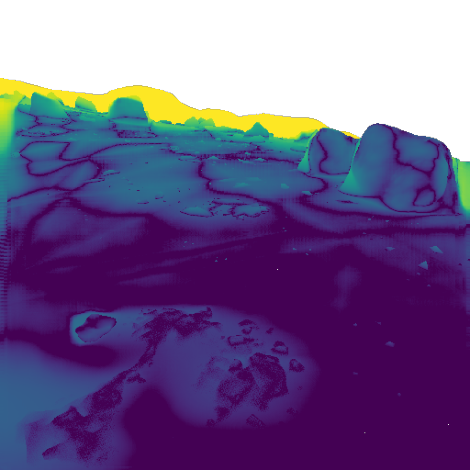
\includegraphics[width=\textwidth]{figures/depth_error_RAFTStereo.png}
		\caption{\bfseries RAFT-Stereo}
	\end{subfigure}\hfill
	\begin{subfigure}[b]{0.16\textwidth}
		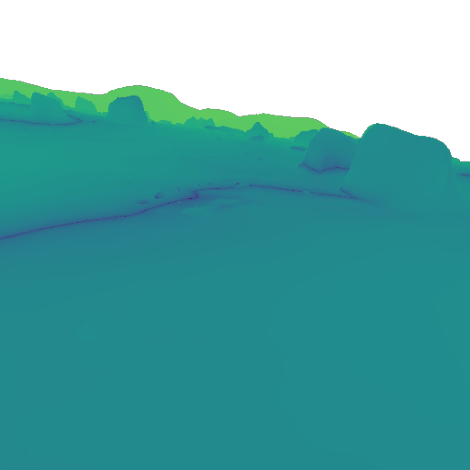
\includegraphics[width=\textwidth]{figures/depth_error_Depth Anything V2 (small).png}
		\caption{\bfseries Depth Anything}
	\end{subfigure}\hfill
	\begin{subfigure}[b]{0.16\textwidth}
		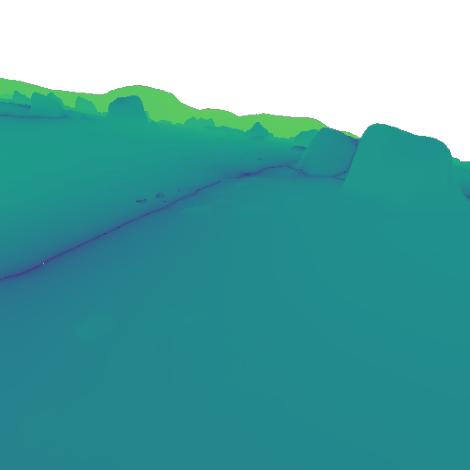
\includegraphics[width=\textwidth]{figures/depth_error_DPT.png}
		\caption{\bfseries DPT}
	\end{subfigure}
	\caption{\bfseries Input image and depth estimation errors for a sample of the LuSNAR dataset~\cite{liu_lusnarlunar_2024}. The other image used for stereo methods is not shown. The errors are in logarithmic scale to qualitatively characterize the performance of the models.}
	\label{fig:depth_errors}
\end{figure*}


\subsection{Evaluation Metrics}
This subsection defines the evaluation metrics used to assess the performance of the proposed framework.

\subsubsection{Depth Estimation}
All depth estimation metrics are computed only over the valid pixels defined by the surface mask, $M_{\text{full}}$. For a rendered depth map $\hat{D}$ and a ground truth depth map $D$:
\begin{itemize}
	\item \textbf{Mean Absolute Error (MAE) [m] $\downarrow$}: The average L1 distance between the rendered and ground truth depth.
	      \begin{equation}
		      \text{MAE} = \frac{1}{|M_{\text{full}}|} \sum_{p \in M_{\text{full}}} |\hat{D}(p) - D(p)|
	      \end{equation}

	\item \textbf{Absolute Relative Error (AbsRel) $\downarrow$}: The scale-invariant average of the absolute relative difference.
	      \begin{equation}
		      \text{AbsRel} = \frac{1}{|M_{\text{full}}|} \sum_{p \in M_{\text{full}}} \frac{|\hat{D}(p) - D(p)|}{D(p)}
	      \end{equation}

	\item \textbf{Threshold Accuracy ($\delta_{25\%}$) $\uparrow$}: The percentage of pixels where the ratio between the rendered and ground truth depth is within a factor of 25\%.
	      \begin{equation}
		      \delta_{25\%} = \frac{1}{|M_{\text{full}}|} \sum_{p \in M_{\text{full}}} \mathbbm{1}\left\{\max\left(\frac{\hat{D}(p)}{D(p)}, \frac{D(p)}{\hat{D}(p)}\right) < 1.25\right\}
	      \end{equation}

	\item \textbf{Frames Per Second (FPS) $\uparrow$}: The processing throughput of the depth estimation model.
\end{itemize}

\subsubsection{Semantic Segmentation}
We compute the following metrics over all the pixels in the image for the semantic segmentation models:
\begin{itemize}
	\item \textbf{Intersection over Union (mIoU) $\uparrow$}: The overlap between the predicted and ground truth masks for a single class or label.
	      \begin{equation}
		      \text{IoU} = \frac{\text{TP}}{\text{TP} + \text{FP} + \text{FN}}
	      \end{equation}

	\item \textbf{Accuracy (Acc.) $\uparrow$}: The percentage of all pixels in the image that are correctly classified.
	      \begin{equation}
		      \text{Acc.} = \frac{\text{TP} + \text{TN}}{\text{TP} + \text{TN} + \text{FP} + \text{FN}}
	      \end{equation}
\end{itemize}

\subsubsection{Surface Reconstruction}
To evaluate the final 3D map, we extract a point cloud, $\hat{P}$, by taking the means of the Gaussians in the dense representation and compare it to the ground truth point cloud, $P$. While a more accurate surface reconstruction could be achieved by leveraging the full density field of the Gaussians, this is beyond the scope of our current work. However, since our map is sufficiently dense, using the means of the Gaussians provides a good approximation for evaluation.
\begin{itemize}
	\item \textbf{Accuracy (Chamfer-$L_2$) [cm] $\downarrow$}: The average distance from each point in the reconstructed point cloud to its nearest neighbor in the ground truth point cloud. This measures the correctness of the reconstructed surface.
	      \begin{equation}
		      \text{Accuracy} = \frac{1}{|\hat{P}|} \sum_{\hat{p} \in \hat{P}} \min_{p \in P} \|\hat{p} - p\|_2
	      \end{equation}

	\item \textbf{Completeness (Chamfer-$L_2$) [cm] $\downarrow$}: The average distance from each point in the ground truth to its nearest neighbor in the reconstruction. This measures how well the reconstruction covers the ground truth surface.
	      \begin{equation}
		      \text{Completeness} = \frac{1}{|P|} \sum_{p \in P} \min_{p \in \hat{P}} \|p - \hat{p}\|_2
	      \end{equation}

	\item \textbf{Precision ($d$) [\%] $\uparrow$}: The percentage of reconstructed points within a distance threshold $d$ of the ground truth, measuring correctness.
	      \begin{equation}
		      \text{Precision}(d) = \frac{1}{|\hat{P}|} \sum_{p \in \hat{P}} \mathbbm{1}\left\{\min_{p \in P} \|p - \hat{p}\|_2 < d\right\}
	      \end{equation}

	\item \textbf{Recall ($d$) [\%] $\uparrow$}: The percentage of ground truth points that have a reconstructed point within a distance threshold $d$, measuring completeness.
	      \begin{equation}
		      \text{Recall}(d) = \frac{1}{|P|} \sum_{p \in P} \mathbbm{1}\left\{\min_{p \in \hat{P}} \|p - \hat{p}\|_2 < d\right\}
	      \end{equation}

	\item \textbf{F1-Score ($d$) [\%] $\uparrow$}: The harmonic mean of Precision and Recall, providing a single metric that balances correctness and completeness.
	      \begin{equation}
		      F_1(d) = 2 \cdot \frac{\text{Precision}(d) \cdot \text{Recall}(d)}{\text{Precision}(d) + \text{Recall}(d)}
	      \end{equation}
\end{itemize}


\subsection{Depth Estimation}
We evaluate the depth estimation models described in \cref{sec:stereo_depth_estimation,sec:monocular_depth_estimation} in the LuSNAR dataset.
\Cref{fig:depth_errors} shows the RGB input and the depth errors for different depth estimation models in logarithmic scale to qualitatively characterize the performance of the models.
Traditional stereo methods like BM and SGBM perform well under favorable illumination conditions but struggle when the light source is behind the camera or when dealing with bright areas and shadows. Learning-based stereo models, particularly RAFT-Stereo, demonstrate superior performance with high depth completion rates and excellent accuracy at short distances. While monocular models lag behind even after proper scaling, achieving error rates comparable to previous models only at medium distances, they could still be valuable for surface reconstruction when combined with proper uncertainty quantification, as they provide significantly more information than RGB images alone.


\Cref{tab:depth_models} shows the quantitative results of the depth estimation models.
Traditional stereo methods achieve low MAE and AbsRel by producing depth only in regions where they are confident, which is evident from their low $\delta_{25\%}$ values. Learning-based stereo models like RAFT-Stereo predict depth more densely, including at longer ranges, which increases MAE due to larger absolute errors at far distances. However, the AbsRel remains comparable, indicating that relative errors remain low across distances. These models also operate at significantly lower frame rates compared to traditional methods. Monocular models underperform across all metrics, even after scale correction, but remain potentially useful when stereo input is not available. Since they are trained on Earth-based datasets, their performance on this terrain requires further evaluation, particularly with respect to finetuning.
\begin{table}[t]
	\centering
	\small
	\caption{\bfseries Comparison of depth estimation models. Monocular depth is scaled using triangulated points from matched features.}
	\label{tab:depth_models}
	\begin{tabular}{|lrrrrr|}
		\hline
		\textbf{Model}                          &
		\textbf{Params}                         &
		\textbf{MAE}$\downarrow$                &
		\textbf{AbsRel}$\downarrow$             &
		\textbf{$\delta_{25\%}$}$\uparrow$      &
		\textbf{FPS}$\uparrow$                                                     \\
		\hline\hline
		\textbf{Stereo}                         &      &      &      &      &      \\
		BM                                      & --   & 1.6  & 0.02 & 0.30 & 24.5 \\
		SGBM                                    & --   & 1.6  & 0.02 & 0.41 & 14.9 \\
		RAFT-Stereo                             & 11M  & 7.3  & 0.05 & 0.72 & 4.5  \\
		CREStereo                               & 5M   & 3.5  & 0.04 & 0.73 & 1.4  \\
		\hline\hline
		\multicolumn{2}{|l}{\textbf{Monocular}} &      &      &      &             \\
		\multicolumn{2}{|l}{Depth Anything V2}  &      &      &      &             \\
		~ Small                                 & 25M  & 11.1 & 0.21 & 0.53 & 13.2 \\
		~ Base                                  & 97M  & 10.8 & 0.19 & 0.56 & 13.2 \\
		~ Large                                 & 335M & 10.7 & 0.18 & 0.59 & 9.8  \\
		GLPN                                    & 61M  & 15.1 & 1.82 & 0.07 & 9.9  \\
		DPT                                     & 343M & 11.2 & 0.19 & 0.55 & 13.6 \\
		Depth Pro                               & 952M & 11.4 & 0.20 & 0.55 & 1.7  \\
		\hline
	\end{tabular}
\end{table}

\cref{fig:depth_stereo_lusnar} shows the performance of RAFT-Stereo. The model shows consistent performance with high accuracy in near regions (below 5 cm error). Precise depth estimates even in challenging lighting conditions and complex geometries.
\begin{figure}[h]
	\centering
	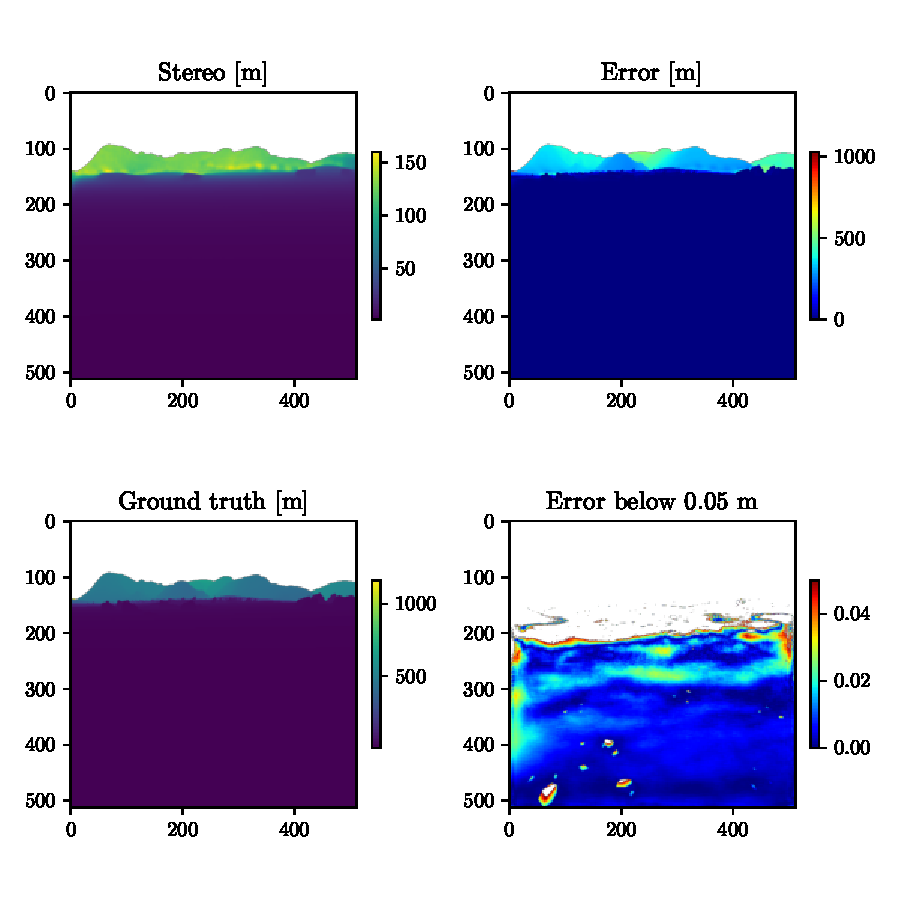
\includegraphics[width=\linewidth]{figures/depth_stereo_lusnar.pdf}
	\caption{\bfseries LuSNAR dataset.}
	\label{fig:depth_stereo_lusnar}
\end{figure}
\begin{figure}[t]
	\centering
	\begin{subfigure}[b]{\linewidth}
		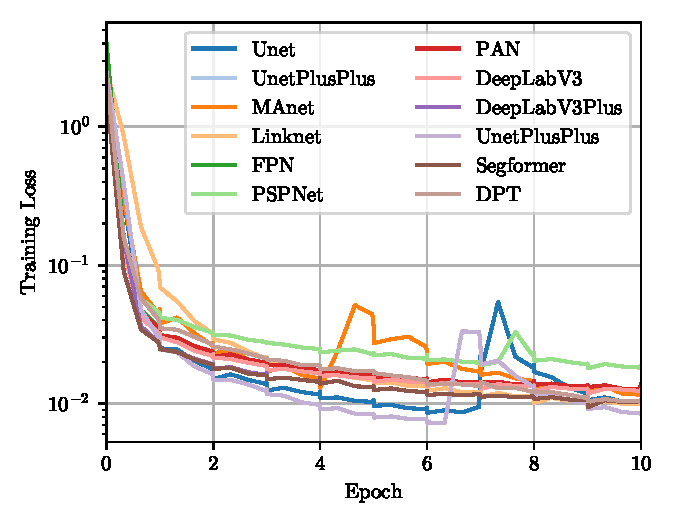
\includegraphics[width=\linewidth]{seg_2d/figures/LuSNAR_losses.pdf}
		\caption{\bfseries Training losses.}
		\label{fig:lusnar_losses}
	\end{subfigure}
	\begin{subfigure}[b]{\linewidth}
		\includegraphics[width=\linewidth]{seg_2d/figures/LuSNAR_losses_val.pdf}
		\caption{\bfseries Validation losses.}
		\label{fig:lusnar_val_losses}
	\end{subfigure}
	\caption{\bfseries Training and validation losses for the considered semantic segmentation models.}
\end{figure}
\begin{figure}[h!]
	\centering
	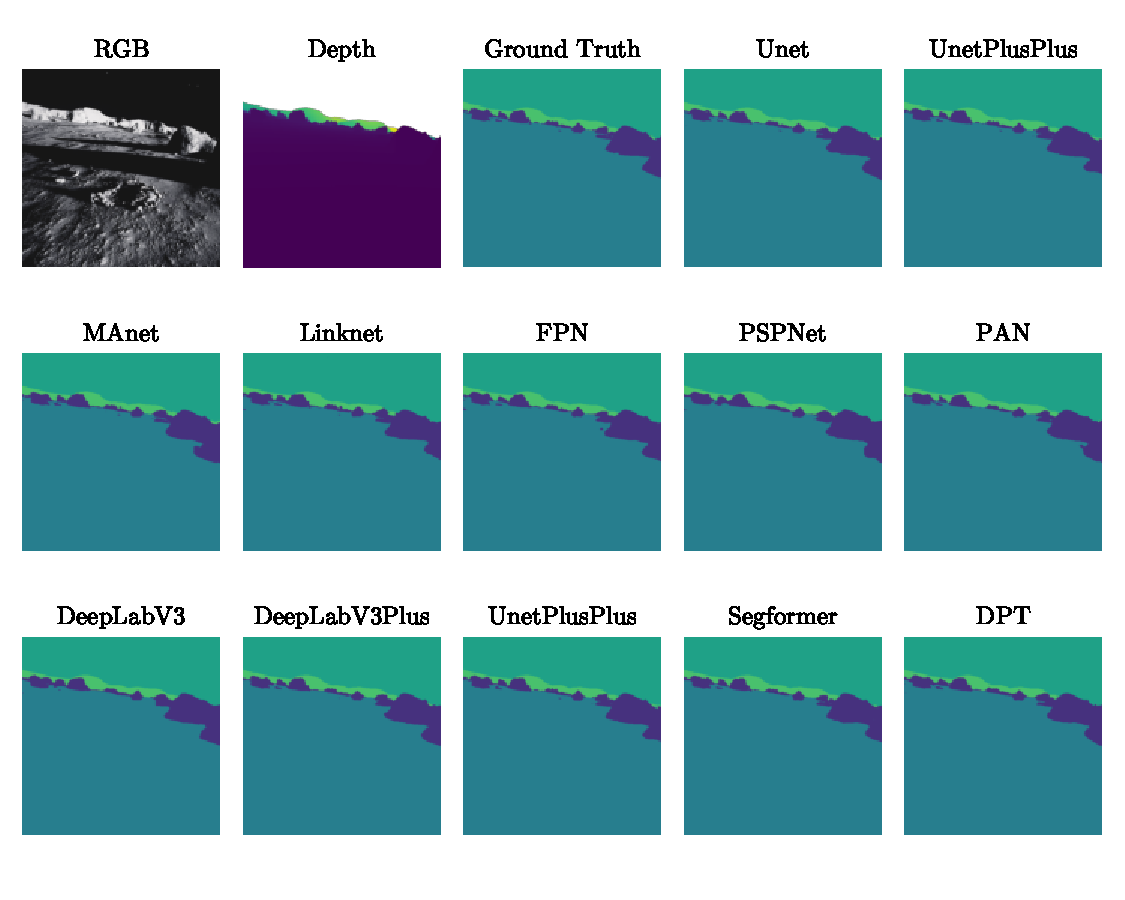
\includegraphics[width=\linewidth, trim={0 0em 0 0em}, clip]{seg_2d/figures/LuSNAR_predictions.pdf}
	\caption{\bfseries Test sample of semantic segmentation predictions for the LuSNAR dataset. Misclassied pixels are highlighted in red.}
	\label{fig:lusnar_predictions}
\end{figure}

\begin{table*}[h!]
	\centering
	\caption{\bfseries Semantic segmentation results on the LuSNAR dataset.}
	\label{tab:semantic_segmentation_models}
	\small
	\begin{tabular}{|l rrrrrrrrrr|}
		\hline
		\multicolumn{1}{|c}{\multirow{2}{*}{\textbf{Model}}}         &
		\multicolumn{1}{c}{\multirow{2}{*}{\textbf{Size [MB]}}}      &
		\multicolumn{1}{c}{\multirow{2}{*}{\textbf{Params}}}         &
		\multicolumn{1}{c}{\multirow{2}{*}{\textbf{FPS $\uparrow$}}} &
		\multicolumn{5}{c}{\textbf{IoU [\%] $\uparrow$}}             &
		\multicolumn{1}{c}{\textbf{Mean}}                            &
		\multicolumn{1}{c|}{\textbf{Mean}}
		\\
		\cmidrule{4-7}
		                                                             &               &               &               &
		\textbf{Regolith}                                            &
		\textbf{Crater}                                              &
		\textbf{Rock}                                                &
		\textbf{Mountain}                                            &
		\textbf{Sky}                                                 &
		\multicolumn{1}{c}{\textbf{IoU $\uparrow$}}                  &
		\multicolumn{1}{c|}{\textbf{Accuracy $\uparrow$}}
		\\
		\hline
		\hline
		U-Net                                                        & 55.0          & 14.3M         &
		114.4                                                        & \textbf{99.5} & 95.5          & 89.2          & 96.5          & \textbf{99.8} & 96.1          & 99.5          \\
		U-Net++                                                      & 61.0          & 16.0M         &
		78.0                                                         & \textbf{99.5} & 91.1          & \textbf{91.6} & \textbf{98.5} & \textbf{99.8} & 96.1          & \textbf{99.6} \\
		MA-Net                                                       & 83.0          & 21.7M         &
		71.7                                                         & 99.2          & 70.9          & 90.1          & 97.5          & \textbf{99.8} & 91.5          & 99.3          \\
		Linknet                                                      & 44.0          & 11.7M         &
		104.5                                                        & 99.2          & 96.4          & 91.1          & 97.0          & \textbf{99.8} & \textbf{96.7} & 99.3          \\
		FPN                                                          & 50.0          & 13.0M         &
		108.7                                                        & 98.9          & \textbf{97.7} & 86.8          & 97.8          & 99.7          & 96.2          & 99.2          \\
		PSPNet                                                       & \textbf{3.0}  & \textbf{0.9M} &
		\textbf{203.2}                                               & 98.8          & 92.7          & 79.7          & 94.3          & 99.6          & 93.0          & 99.0          \\
		PAN                                                          & 43.0          & 11.4M         &
		92.8                                                         & 99.0          & 94.6          & 84.3          & 97.4          & 99.7          & 95.0          & 99.2          \\
		DeepLabV3                                                    & 61.0          & 15.9M         &
		131.5                                                        & 99.0          & 96.7          & 86.6          & 98.3          & 99.7          & 96.1          & 99.2          \\
		DeepLabV3Plus                                                & 47.0          & 12.3M         &
		118.8                                                        & 99.2          & 96.4          & 89.2          & 98.0          & \textbf{99.8} & 96.5          & 99.4          \\
		Segformer                                                    & 45.0          & 11.8M         &
		140.5                                                        & 99.2          & 95.5          & 88.9          & 97.7          & \textbf{99.8} & 96.2          & 99.4          \\
		DPT                                                          & 159.0         & 41.6M         &
		79.6                                                         & 99.1          & 94.1          & 87.4          & 95.7          & 99.7          & 95.2          & 99.3          \\
		\hline
	\end{tabular}
\end{table*}

\subsection{Semantic Segmentation}
We benchmarked a suite of semantic segmentation architectures on the LuSNAR dataset to evaluate their effectiveness for lunar terrain classification. All models were trained to classify five semantic categories present in the dataset: regolith, craters, rocks, mountains, and sky~\cite{liu_lusnarlunar_2024}. The dataset was split into approximately 8,000 images for training, 1,000 for validation, and 2,000 for testing. For training, we used the Adam optimizer over 10 epochs with a batch size of 24. The initial learning rate was $1\times10^{-3}$, which was adjusted by a scheduler that reduced the rate by a factor of 0.75 with a patience of 10 epochs, down to a minimum of $1\times10^{-7}$.

As shown by the training and validation loss curves in \Cref{fig:lusnar_losses,fig:lusnar_val_losses}, all models converged successfully. Qualitatively, the majority of architectures are able to accurately segment the primary terrain features, with representative examples shown in \Cref{fig:lusnar_predictions}. The quantitative results in \Cref{tab:semantic_segmentation_models} reveal key performance trade-offs. While models like LinkNet and DeepLabV3+ achieve high overall mean IoU, other models excel at specific classes critical for navigation; for instance, FPN is the most effective at crater detection. Notably, PSPNet offers a highly efficient solution, achieving the highest FPS with by far the smallest model size, making it a strong candidate for resource-constrained hardware.
For our downstream mapping task, we selected U-Net++ due to having the best overall accuracy and IoU for rocks (91.6\% IoU), a critical capability for ensuring rover safety, while being computationally comparable to the other models.

% \begin{figure}[h]
%     \centering
%     \begin{subfigure}[b]{\linewidth}
%         \centering
%         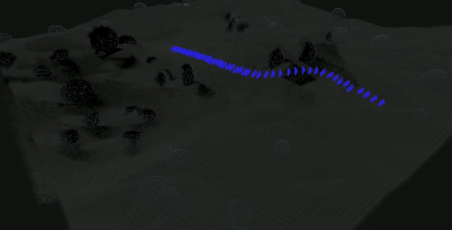
\includegraphics[width=0.8\textwidth]{gaussians_1.png}
%         \caption{\bfseries Ground truth depth and segmentation.}
%         \label{fig:gaussians_1}
%     \end{subfigure}
%     \begin{subfigure}[b]{\linewidth}
%         \centering
%         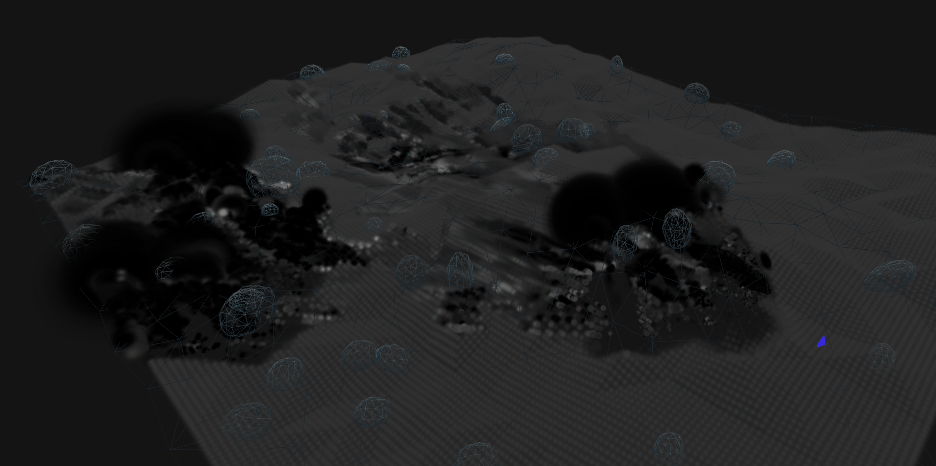
\includegraphics[width=0.8\textwidth]{gaussians_3.png}
%         \caption{\bfseries RAFT-Stereo depth and U-Net++ segmentation.}
%         \label{fig:gaussians_3}
%     \end{subfigure}
%     \caption{\bfseries Effect of depth estimation and segmentation on 3D Gaussian Splatting.}
% \end{figure}

\begin{figure}[b!]
	\centering
	\begin{subfigure}[b]{0.49\linewidth}
		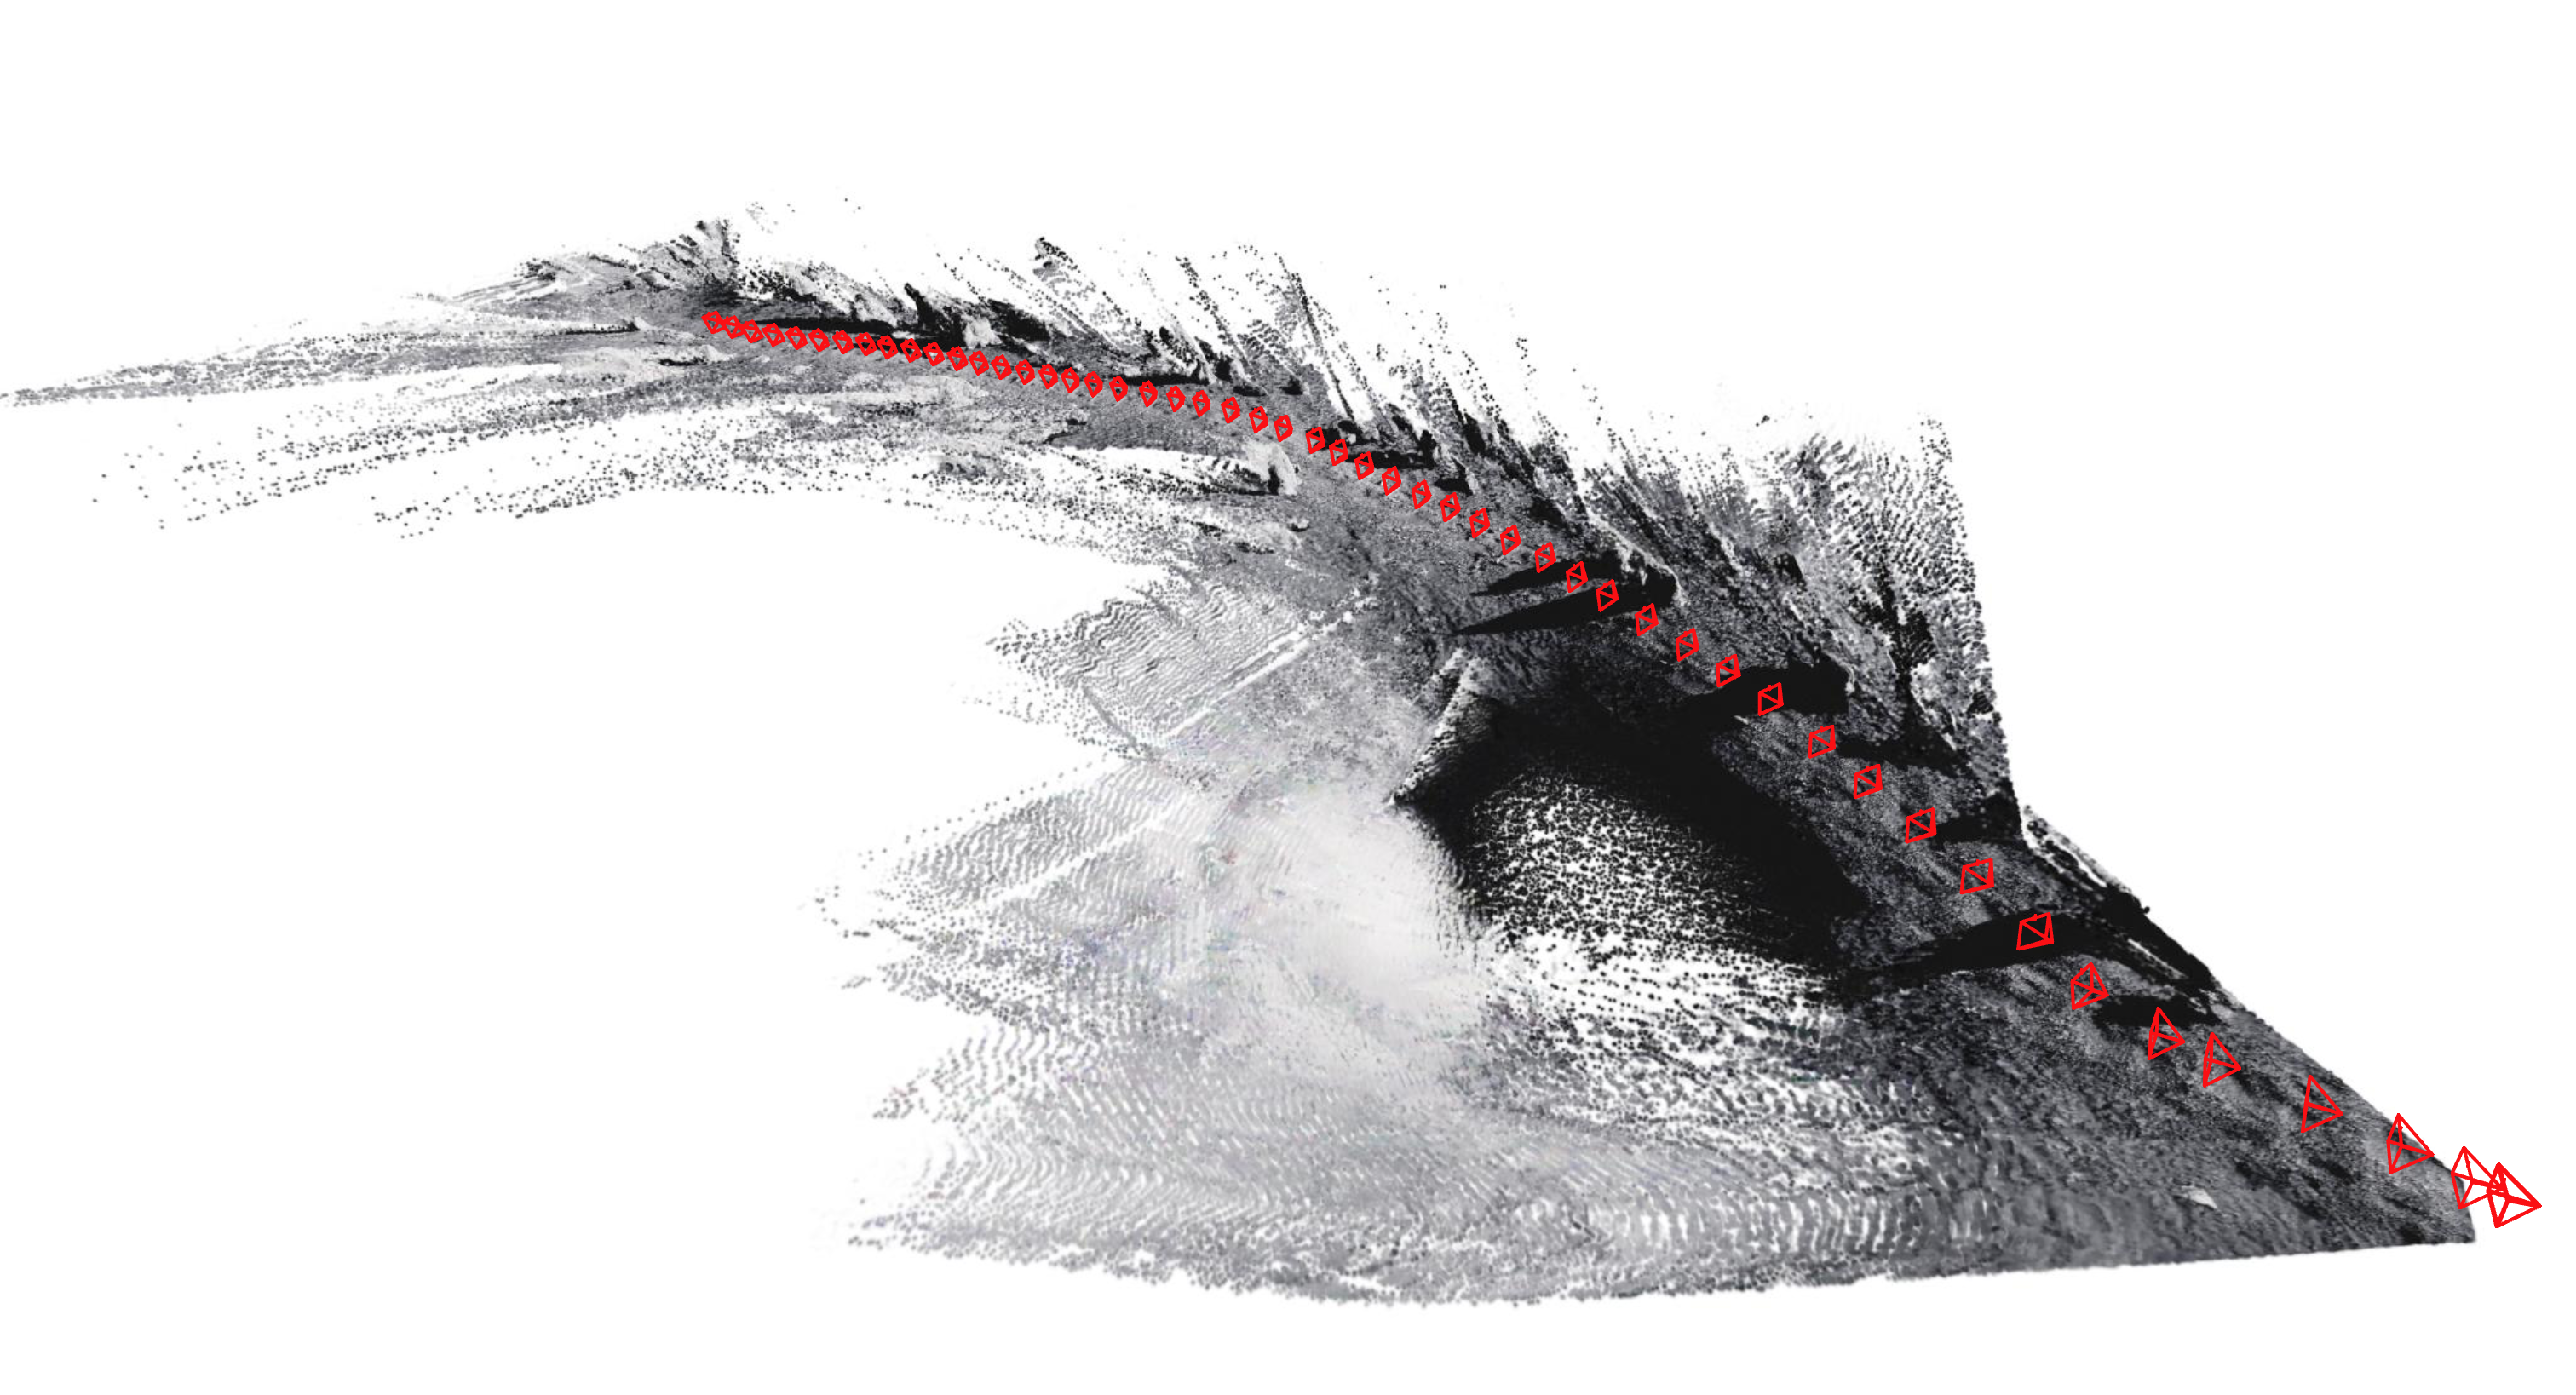
\includegraphics[width=\linewidth]{figures/3dgs/render-partial-rgb.png}
		\caption{\bfseries Initial map (RGB).}
	\end{subfigure}
	\hfill
	\begin{subfigure}[b]{0.49\linewidth}
		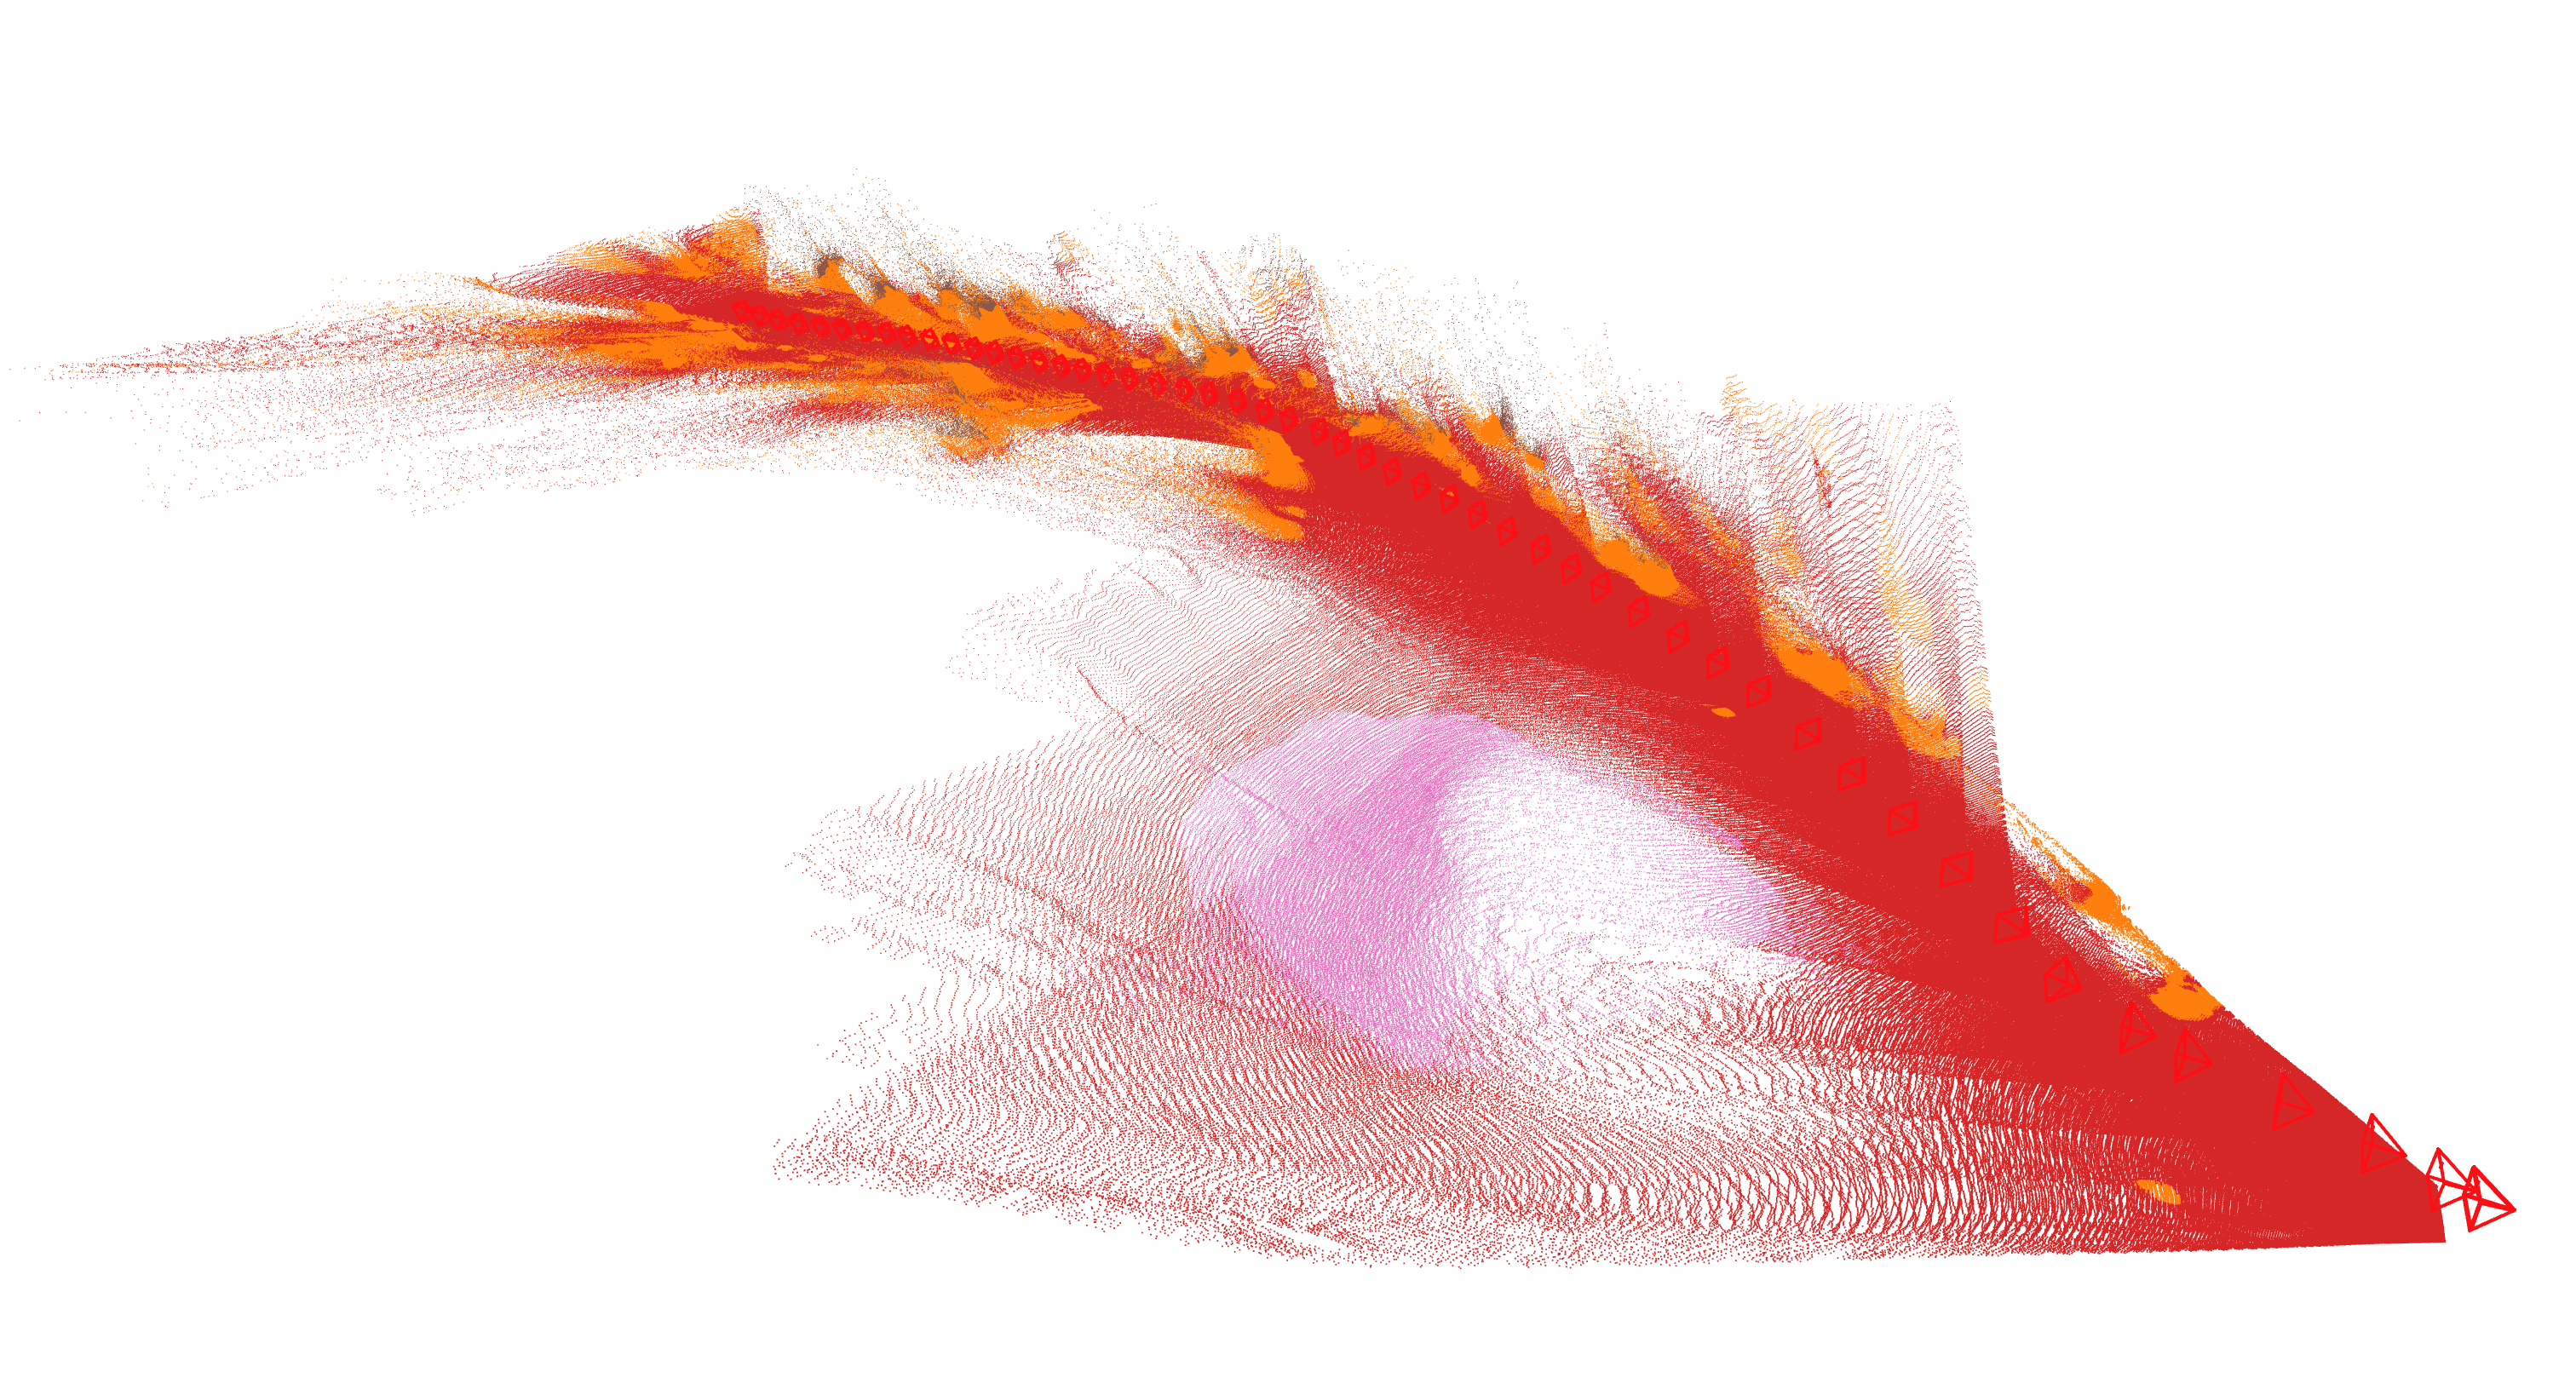
\includegraphics[width=\linewidth]{figures/3dgs/render-partial-semantic.png}
		\caption{\bfseries Partial map (semantic).}
	\end{subfigure}
	\begin{subfigure}[b]{\linewidth}
		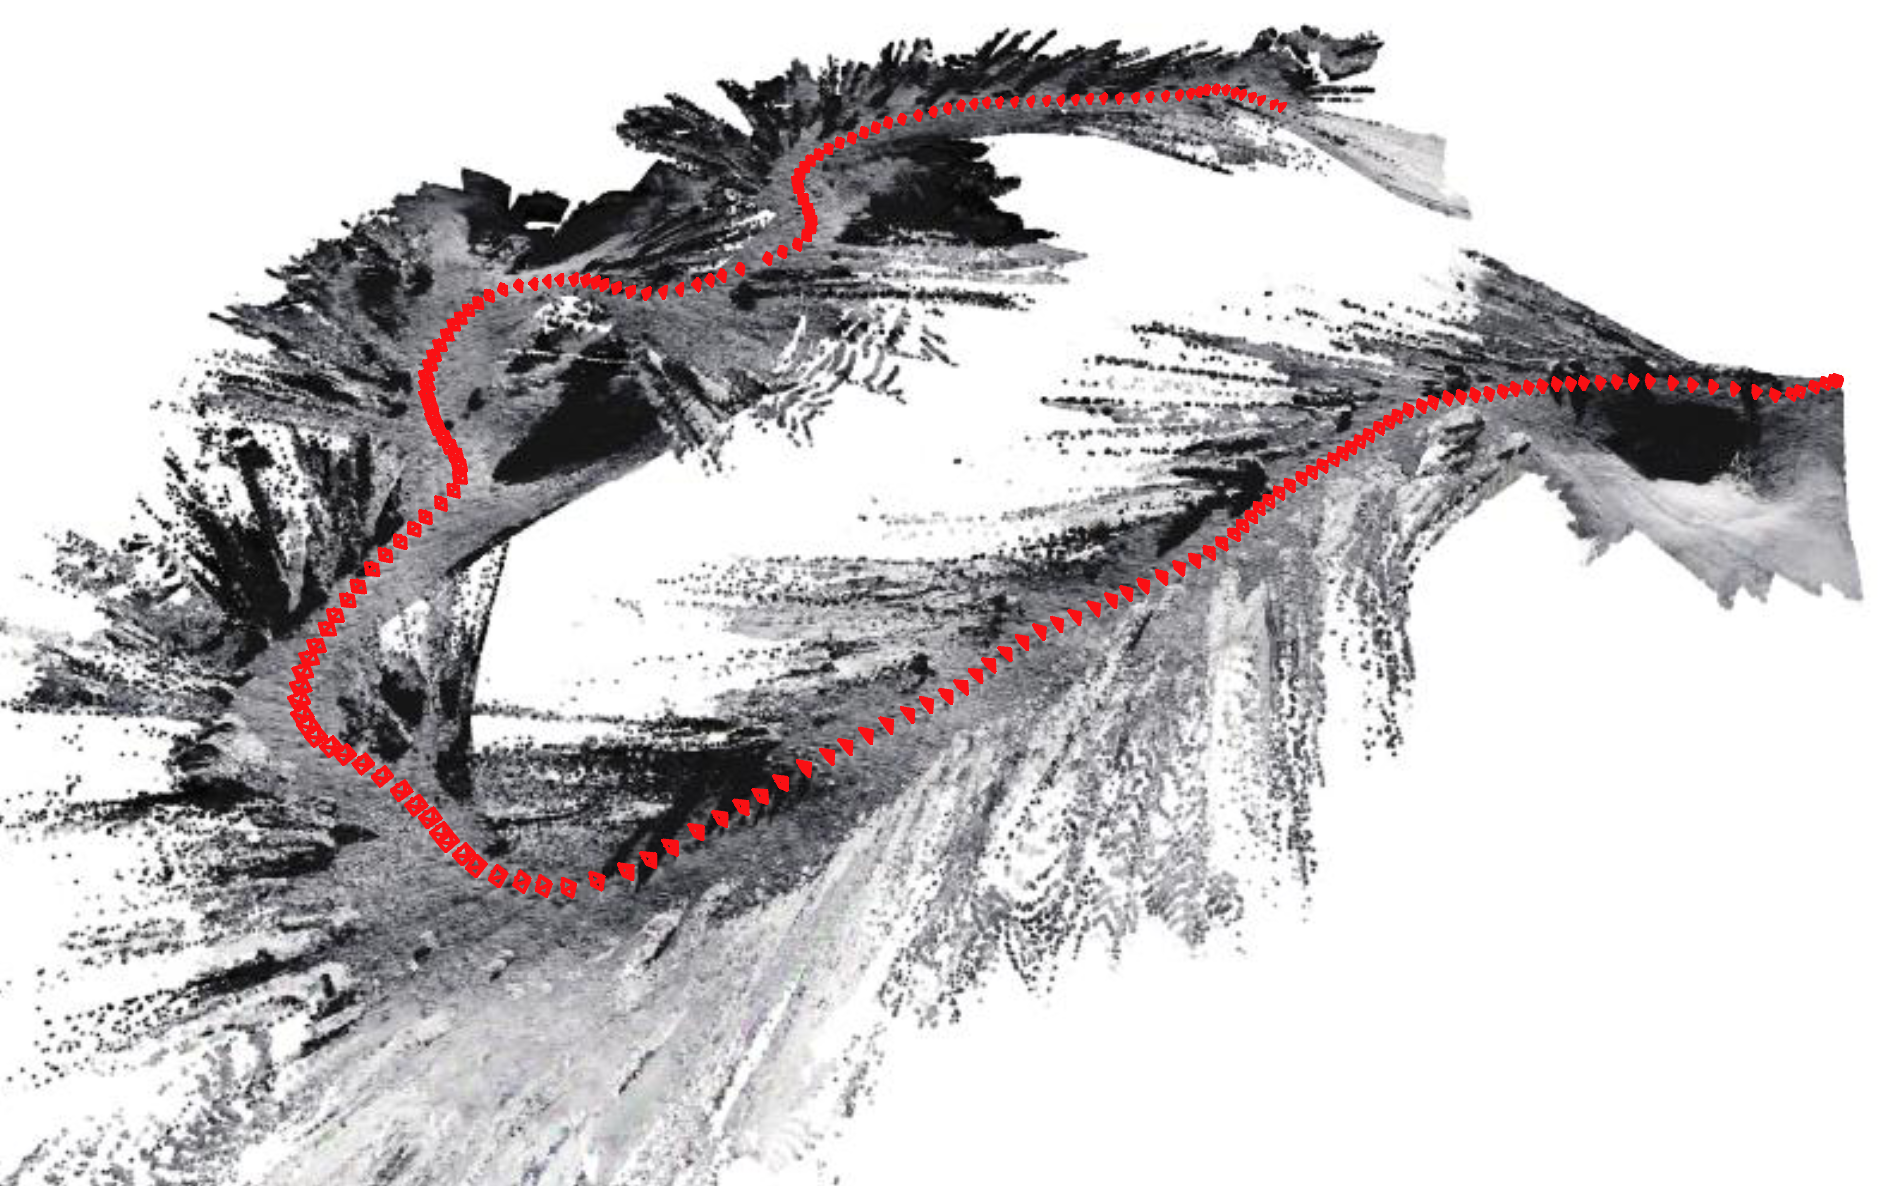
\includegraphics[width=\linewidth,trim=0 0 0 0,clip]{figures/3dgs/render-full.png}
		\caption{\bfseries Final map (RGB).}
	\end{subfigure}
	\caption{\bfseries Partial and final 3DGS maps.}
	\label{fig:map_3dgs}
\end{figure}

\begin{figure*}[t]
	\centering
	\begin{subfigure}[b]{0.3\linewidth}
		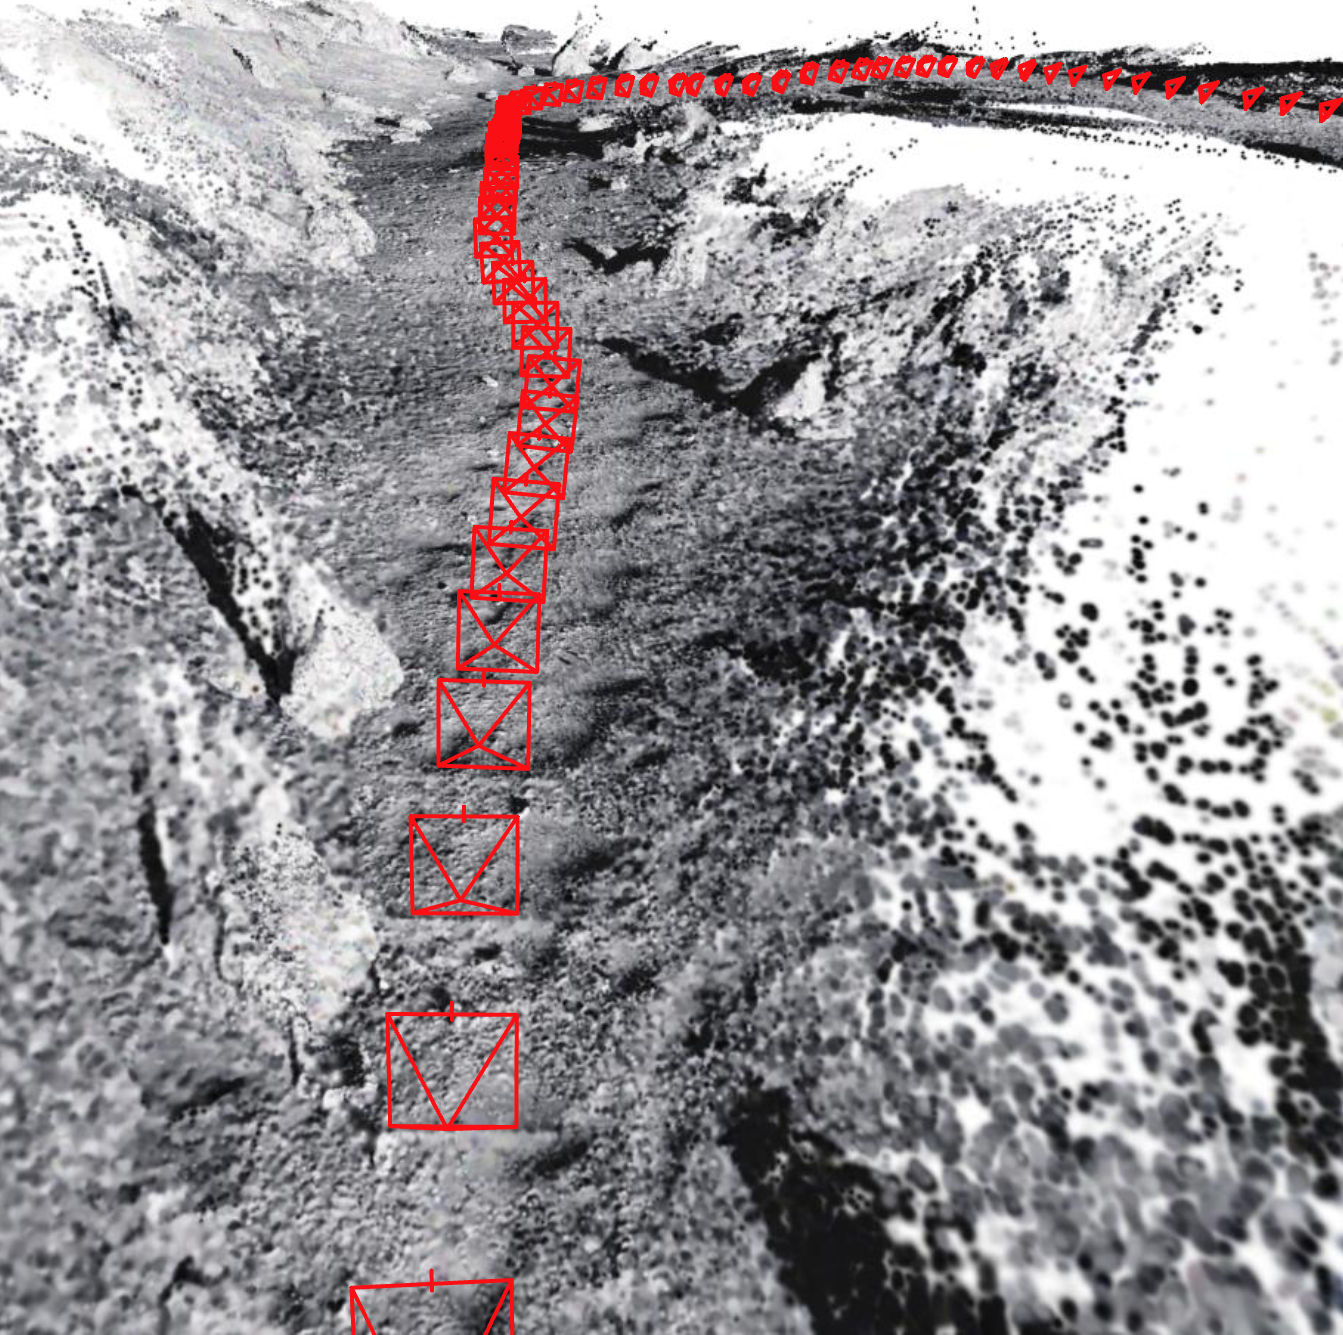
\includegraphics[width=\linewidth]{figures/3dgs/render-birdseye.png}
	\end{subfigure}
	\hfill
	\begin{subfigure}[b]{0.3\linewidth}
		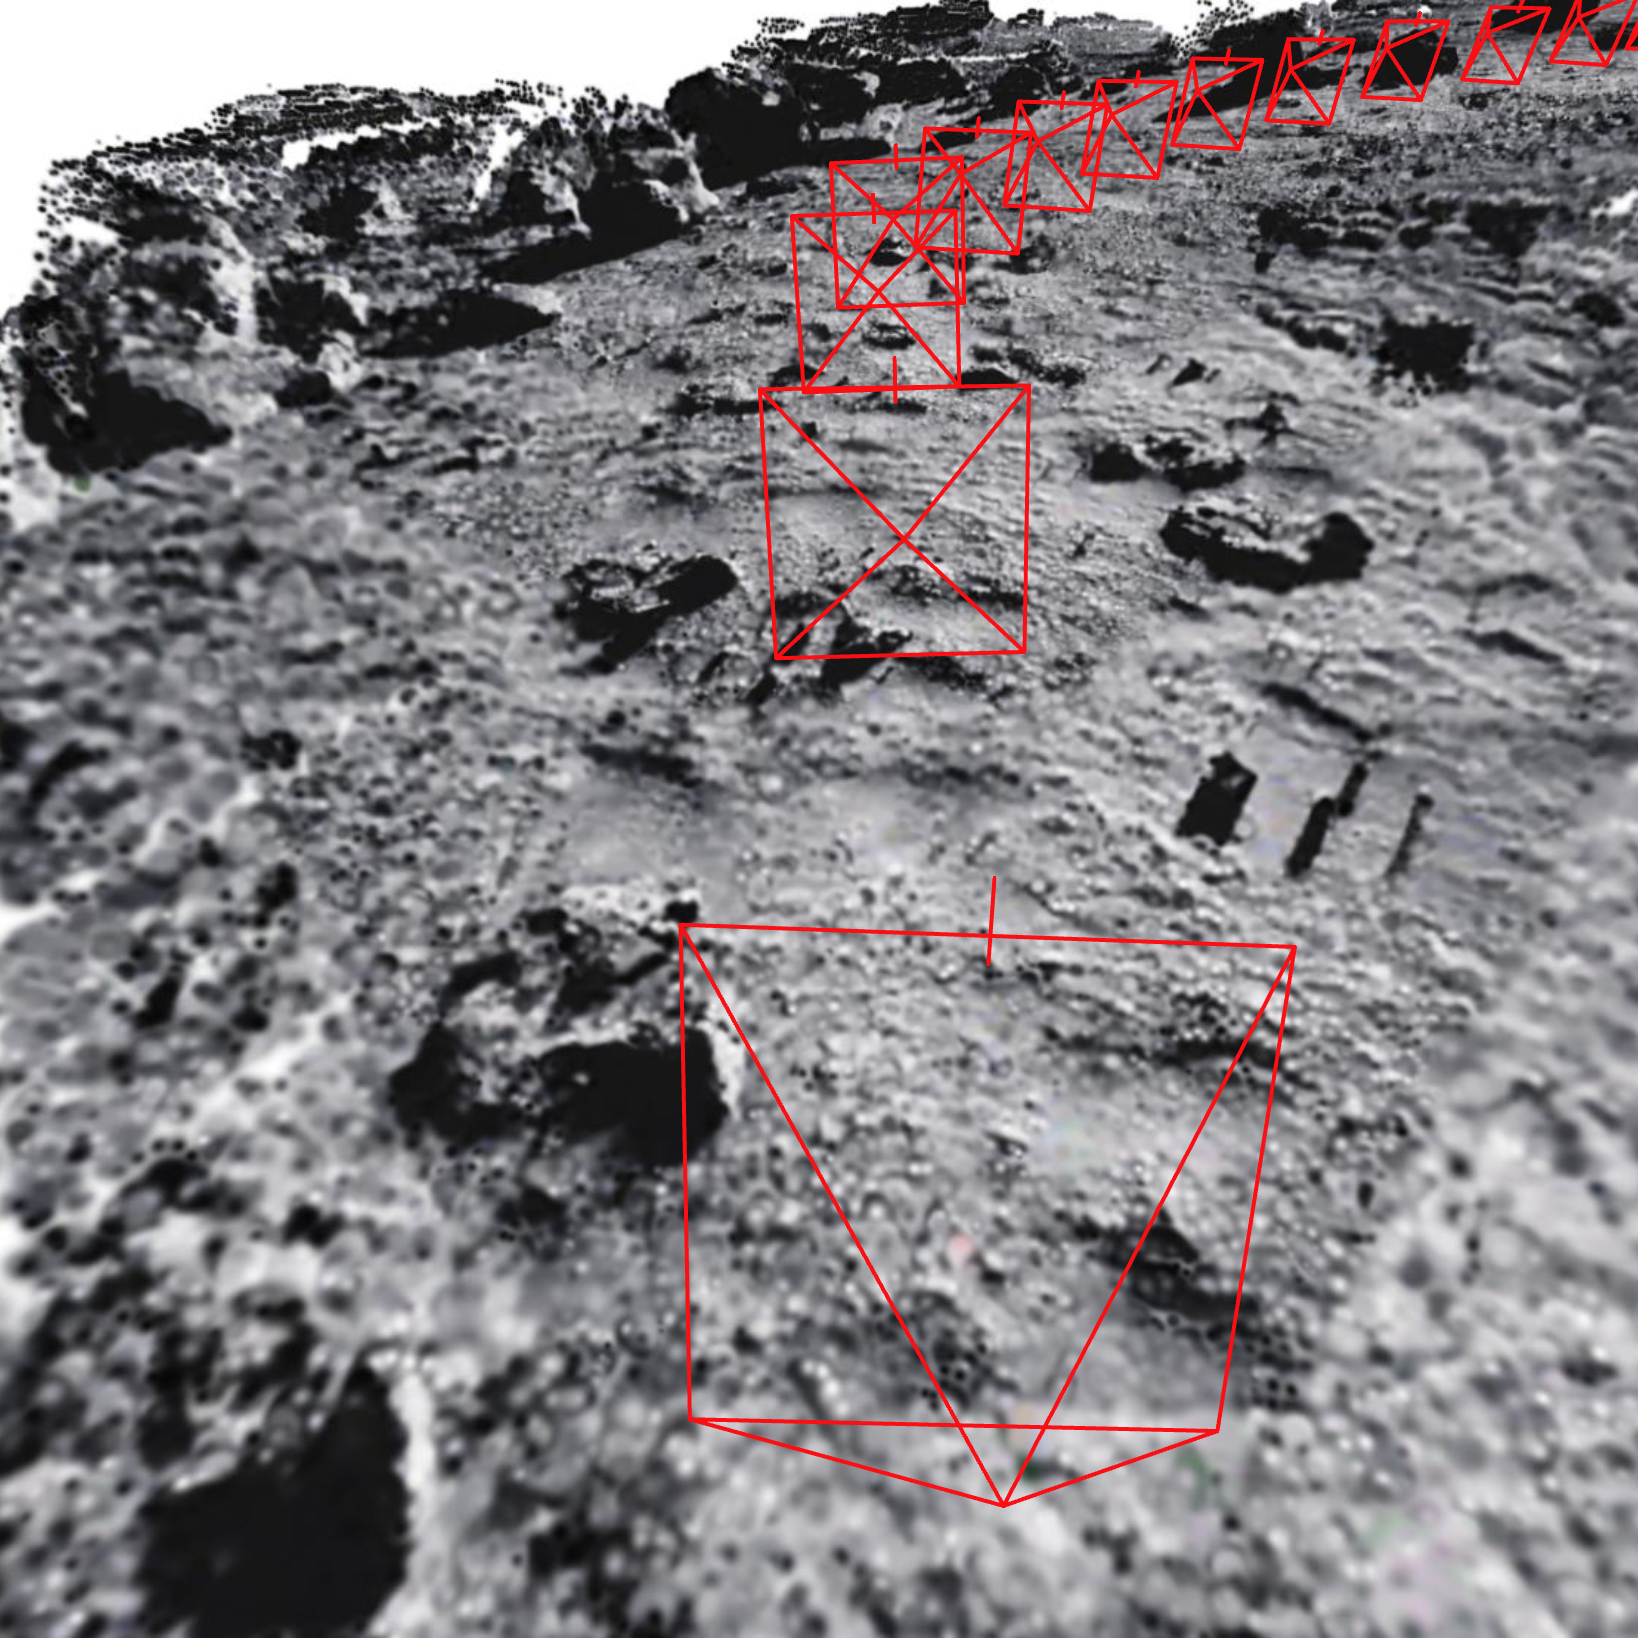
\includegraphics[width=\linewidth,trim=10em 0 0 0,clip]{figures/3dgs/render-close.png}
	\end{subfigure}
	\hfill
	\begin{subfigure}[b]{0.3\linewidth}
		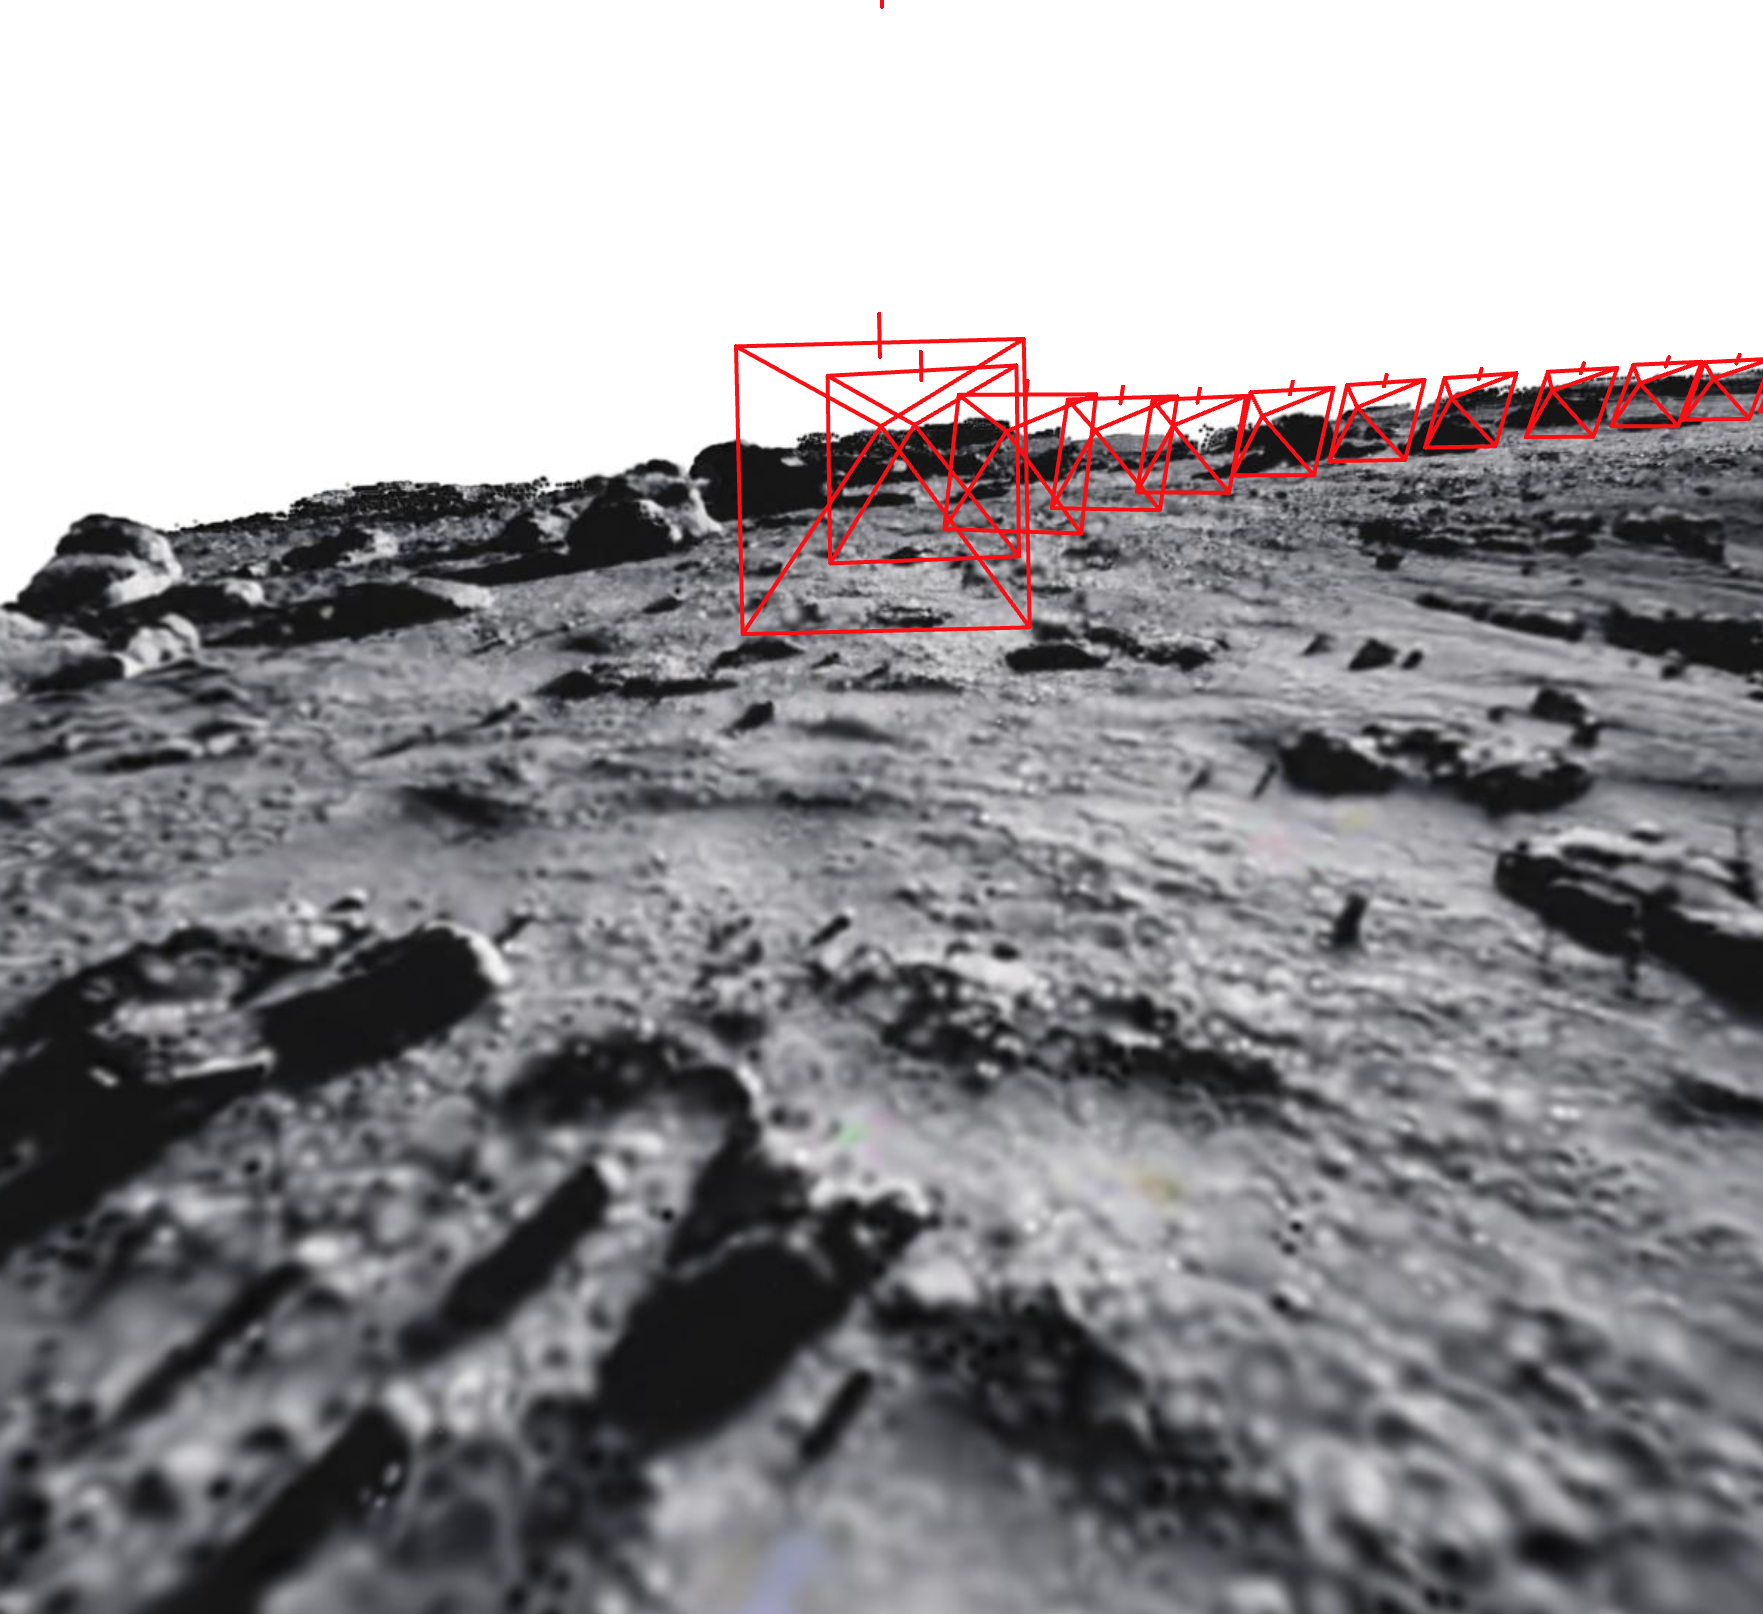
\includegraphics[width=\linewidth]{figures/3dgs/render-camera.png}
	\end{subfigure}
	\caption{\bfseries Qualitative novel view synthesis results rendered from the 3DGS map.}
	\label{fig:novel_views}
\end{figure*}

\begin{table*}[h]
	\centering
	\small
	\caption{\bfseries Summary of surface reconstruction results. Precision and recall using a threshold of 10 cm.}
	\label{tab:surface_reconstruction_short}
	\begin{tabular}[t]{|lrrrrrr|}
		\hline
		\multirow{2}{*}{\textbf{Metric}}               &
		\multicolumn{1}{c}{\textbf{Accuracy}}          &
		\multicolumn{1}{c}{\textbf{Completion}}        &
		\multicolumn{1}{c}{\textbf{Precision}}         &
		\multicolumn{1}{c}{\textbf{Recall}}            &
		\multicolumn{1}{c}{\textbf{F-Score}}           &
		\multicolumn{1}{c|}{\textbf{Height Error}}
		\\
		\multicolumn{1}{|c}{}                          &
		\multicolumn{1}{c}{\textbf{[cm] $\downarrow$}} &
		\multicolumn{1}{c}{\textbf{[cm] $\downarrow$}} &
		\multicolumn{1}{c}{\textbf{[\%] $\uparrow$}}   &
		\multicolumn{1}{c}{\textbf{[\%] $\uparrow$}}   &
		\multicolumn{1}{c}{\textbf{[\%] $\uparrow$}}   &
		\multicolumn{1}{c|}{\textbf{[cm] $\downarrow$}}                                          \\
		\hline\hline
		3DGS                                           & 19.4 & 25.8 & 73.1 & 78.9 & 75.9 & 10.8 \\
		+ GT Segmentation                              & 19.4 & 25.8 & 73.1 & 78.8 & 75.9 & 10.8 \\
		+ GT Depth                                     & 13.3 & 29.4 & 82.3 & 81.1 & 81.7 & 6.0  \\
		+ GT Depth + GT Segmentation                   & 13.3 & 29.4 & 82.3 & 81.1 & 81.7 & 6.0  \\
		\hline
		Point Cloud                                    & 19.2 & 26.0 & 77.1 & 78.0 & 77.5 & 9.8  \\
		+ GT Segmentation                              & 19.2 & 26.0 & 77.1 & 78.0 & 77.5 & 9.8  \\
		+ GT Depth                                     & 12.5 & 29.8 & 89.5 & 81.0 & 85.1 & 4.2  \\
		+ GT Depth + GT Segmentation                   & 12.5 & 29.8 & 89.5 & 81.0 & 85.1 & 4.2  \\
		\hline
	\end{tabular}
\end{table*}

\subsection{Surface Reconstruction}
% Intro
We evaluate our real-time mapping framework on a 500-meter traverse within a scene from the LuSNAR dataset. The input is sourced from a single front-facing stereo camera pair (512x512 pixel resolution) at a rate of 1 Hz. The pipeline uses U-Net++ for semantic segmentation and RAFT-Stereo for dense depth estimation.
We use a ground truth map sampled of 1 cm resolution.
To benchmark our method and selection of perception models, we compare the reconstruction accuracy of this full pipeline against a configuration that uses ground truth depth and segmentation. For this evaluation, we assume ground truth poses are provided, as our primary focus is to analyze the mapping feasibility and performance independent of a front-end tracking system.

% Note on surface reconstruction metrics
For this preliminary analysis, it is important to note how the surface reconstruction metrics are computed. We extract a point cloud from the 3DGS map by using only the position of each Gaussian. This approach is a simplification, as the center of a Gaussian is not constrained to lie directly on the physical surface. By treating the Gaussians as discrete points, we do not yet leverage the continuous, density-based surface representation that is a key advantage of the method~\cite{wolf_gs2mesh_2025}. We are currently developing a more accurate surface reconstruction pipeline that will use this density information to provide a better evaluation of the map's quality.

% Qualitative results
\Cref{fig:map_3dgs} shows the output of the mapping process, displaying a partial 3DGS map that visualizes the semantic information embedded within each Gaussian, as well as the final, complete map for the entire traverse. The quality of the scene representation is further demonstrated in \Cref{fig:novel_views}, which presents novel view synthesis results. These images are rendered from viewpoints that were not seen during the mapping process, highlighting the framework's ability to build a coherent and renderable 3D model of the environment.

% Quantitative results
The quantitative results for the map reconstruction are presented in \Cref{tab:surface_reconstruction,tab:surface_reconstruction_short}. The first table provides a detailed breakdown of performance for each semantic class, while the second summarizes the average results across all classes. From these aggregate results, our full pipeline achieves a mean height error of 10 cm. With a 10 cm evaluation threshold, the precision and recall metrics are over 70\%, indicating that the majority of the reconstructed surface is geometrically consistent with the ground truth.

A key finding is the minimal impact of the segmentation model's accuracy on the final geometry; using ground truth semantic labels resulted in negligible changes to the aggregate metrics, demonstrating the high performance of the U-Net++ model. The per-class breakdown in \Cref{tab:surface_reconstruction} reveals that reconstruction errors are largest for the crater category. This is an expected outcome, as craters in the trajectory are typically distant from the rover and are often poorly illuminated within deep shadows, making accurate depth estimation challenging.
A qualitative analysis of the reconstruction shows that the largest geometric errors are concentrated along the dark, high-contrast edges of rocks. These regions represent a common failure mode for both the depth estimation and semantic segmentation models, which struggle to distinguish shadowed rock boundaries from the dark sky or shadowed regolith.

When using estimated depth under ideal pose conditions, the 3DGS pipeline's performance is quantitatively similar to the point cloud baseline, with the cm-level difference in average height error falling close to the 1 cm resolution of the ground truth map. Our next analysis will explore more challenging scenarios, such as re-mapping the same area to evaluate consistency or introducing pose noise. We hypothesize that in such cases, the 3DGS framework's ability to jointly optimize both the map and camera poses to achieve multi-view consistency would demonstrate a significant advantage.

% Memory usage
\Cref{tab:memory_usage_3dgs} and \Cref{tab:memory_usage_point_cloud} show the memory requirements for the 500-meter traverse, resulting in a map of approximately 15 million Gaussians and 12 million points. It is important to note that the current memory usage can be significantly reduced, as techniques for pruning and compressing the 3DGS map, keyframe buffer, and baseline point cloud are left as future work~\cite{bagdasarian_3dgszip_2025}. The 3DGS map representation itself (775 MB) is more compact than the sum of the images taken RGB (2x1200 MB), indicating that the 3DGS map can become a memory efficient alternative that offers rendering capabilities.

Compared to a traditional semantic point cloud of similar scale, the 3DGS map requires about 2.5 times more memory (336 MB for the point cloud). However, the memory footprint of our framework is highly dependent on the configuration. Only a small subset of the keyframe buffer storing RGB images, depths, and masks is necessary for global optimization tasks like loop closure or refining past poses.
Similarly, the memory for strategy variables is only required for visible Gaussians and can be pruned for areas of the map no longer in view, substantially reducing the active memory load.
Further analysis and optimization of the framework's memory and computational requirements is an area of ongoing work. We are investigating compression techniques for both the 3D Gaussian representation and the keyframe buffer to substantially reduce the memory footprint for long-range traverses.



\begin{table*}[h]
	\centering
	\small
	\begin{minipage}[t]{0.68\linewidth}
		\centering
		\caption{3DGS memory usage.}
		\label{tab:memory_usage_3dgs}
		\centering
		\begin{tabular}[t]{|lrlr|lr|}
			\hline
			\textbf{GPU VRAM} &        &                   & 995 MB & \textbf{System RAM} & 1900 MB \\
			\hline\hline
			\textbf{3DGS}     & 830 MB & \textbf{Strategy} & 165 MB & \textbf{Buffer}     & 1900 MB \\
			~~Rotations       & 222 MB & ~~Radii           & 55 MB  & ~~RGBs              & 1200 MB \\
			~~Means           & 166 MB & ~~Gradients       & 55 MB  & ~~Depths            & 400 MB  \\
			~~Scales          & 166 MB & ~~Counts          & 55 MB  & ~~Masks             & 200 MB  \\
			~~Features        & 166 MB &                   &        & ~~Labels            & 100 MB  \\
			~~Opacities       & 55 MB  &                   &        &                     &         \\
			~~Labels          & 55 MB  &                   &        &                     &         \\
			\hline
		\end{tabular}
	\end{minipage}%
	\begin{minipage}[t]{0.3\linewidth}
		\centering
		\caption{Point Cloud memory usage.}
		\label{tab:memory_usage_point_cloud}
		\begin{tabular}[t]{|lr|}
			\hline
			\textbf{System RAM} & 336 MB \\\hline\hline
			~~Points            & 144 MB \\
			~~Color             & 144 MB \\
			~~Label             & 48 MB  \\\hline
		\end{tabular}
	\end{minipage}
\end{table*}



\begin{table*}[h]
	\centering
	\small
	\caption{\bfseries Surface reconstruction results. Precision and recall using a threshold of 10 cm.}
	\label{tab:surface_reconstruction}
	\begin{tabular}[t]{|lrrrrrr|}
		\hline
		\multirow{2}{*}{\textbf{Metric}}               &
		\multicolumn{1}{c}{\textbf{Accuracy}}          &
		\multicolumn{1}{c}{\textbf{Completion}}        &
		\multicolumn{1}{c}{\textbf{Precision}}         &
		\multicolumn{1}{c}{\textbf{Recall}}            &
		\multicolumn{1}{c}{\textbf{F-Score}}           &
		\multicolumn{1}{c|}{\textbf{Height Error}}
		\\
		\multicolumn{1}{|c}{}                          &
		\multicolumn{1}{c}{\textbf{[cm] $\downarrow$}} &
		\multicolumn{1}{c}{\textbf{[cm] $\downarrow$}} &
		\multicolumn{1}{c}{\textbf{[\%] $\uparrow$}}   &
		\multicolumn{1}{c}{\textbf{[\%] $\uparrow$}}   &
		\multicolumn{1}{c}{\textbf{[\%] $\uparrow$}}   &
		\multicolumn{1}{c|}{\textbf{[cm] $\downarrow$}}                                           \\ \hline\hline
		\multicolumn{7}{|l|}{\textbf{3DGS}}                                                       \\ \hline
		Rock                                           & 64.6  & 27.0 & 22.9 & 56.9 & 32.6 & 16.2 \\
		Regolith                                       & 14.5  & 28.0 & 81.8 & 82.0 & 81.9 & 8.5  \\
		Crater                                         & 944.7 & 27.1 & 13.2 & 41.5 & 20.0 & 75.3 \\
		All                                            & 19.4  & 25.8 & 73.1 & 78.9 & 75.9 & 10.8 \\
		\hline
		\multicolumn{7}{|l|}{\textbf{+ GT Segmentation}}                                          \\ \hline
		Rock                                           & 64.7  & 26.5 & 23.0 & 56.8 & 32.7 & 16.3 \\
		Regolith                                       & 14.4  & 28.0 & 81.8 & 82.0 & 81.9 & 8.5  \\
		Crater                                         & 936.2 & 27.6 & 13.4 & 41.4 & 20.2 & 75.1 \\
		All                                            & 19.4  & 25.8 & 73.1 & 78.8 & 75.9 & 10.8 \\
		\hline
		\multicolumn{7}{|l|}{\textbf{+ GT Depth}}                                                 \\ \hline
		Rock                                           & 29.5  & 34.4 & 51.6 & 55.3 & 53.4 & 7.5  \\
		Regolith                                       & 10.2  & 30.0 & 87.3 & 85.2 & 86.2 & 5.3  \\
		Crater                                         & 384.3 & 47.5 & 42.0 & 73.3 & 53.4 & 42.0 \\
		All                                            & 13.3  & 29.4 & 82.3 & 81.1 & 81.7 & 6.0  \\
		\hline
		\multicolumn{7}{|l|}{\textbf{+ GT Depth + GT Segmentation}}                               \\ \hline
		Rock                                           & 27.7  & 35.5 & 52.1 & 55.5 & 53.8 & 7.4  \\
		Regolith                                       & 10.0  & 30.5 & 87.5 & 85.4 & 86.4 & 5.2  \\
		Crater                                         & 344.5 & 48.8 & 43.2 & 73.4 & 54.4 & 40.8 \\
		All                                            & 13.3  & 29.4 & 82.3 & 81.1 & 81.7 & 6.0  \\ \hline\hline
		\multicolumn{7}{|l|}{\textbf{Point Cloud}}                                                \\ \hline
		Rock                                           & 64.3  & 27.9 & 25.7 & 55.2 & 35.1 & 15.9 \\
		Regolith                                       & 13.6  & 28.1 & 87.2 & 81.6 & 84.3 & 7.0  \\
		Crater                                         & 975.5 & 27.1 & 15.1 & 44.9 & 22.6 & 74.7 \\
		All                                            & 19.2  & 26.0 & 77.1 & 78.0 & 77.5 & 9.8  \\
		\hline
		\multicolumn{7}{|l|}{\textbf{+ GT Segmentation}}                                          \\ \hline
		Rock                                           & 64.4  & 27.5 & 25.8 & 55.4 & 35.2 & 16.0 \\
		Regolith                                       & 13.6  & 28.1 & 87.2 & 81.7 & 84.3 & 7.0  \\
		Crater                                         & 967.1 & 27.6 & 15.4 & 44.8 & 22.9 & 74.4 \\
		All                                            & 19.2  & 26.0 & 77.1 & 78.0 & 77.5 & 9.8  \\
		\hline
		\multicolumn{7}{|l|}{\textbf{+ GT Depth}}                                                 \\ \hline
		Rock                                           & 29.9  & 35.9 & 66.0 & 55.1 & 60.1 & 6.4  \\
		Regolith                                       & 8.7   & 30.1 & 93.5 & 85.0 & 89.0 & 3.3  \\
		Crater                                         & 406.2 & 47.7 & 47.9 & 77.9 & 59.3 & 42.5 \\
		All                                            & 12.5  & 29.8 & 89.5 & 81.0 & 85.1 & 4.2  \\
		\hline
		\multicolumn{7}{|l|}{\textbf{+ GT Depth + GT Segmentation}}                               \\ \hline
		Rock                                           & 27.8  & 37.0 & 67.2 & 55.1 & 60.6 & 6.3  \\
		Regolith                                       & 8.4   & 30.6 & 93.7 & 85.2 & 89.3 & 3.1  \\
		Crater                                         & 365.6 & 49.2 & 49.4 & 77.9 & 60.4 & 41.0 \\
		All                                            & 12.5  & 29.8 & 89.5 & 81.0 & 85.1 & 4.2  \\
		\hline
	\end{tabular}
\end{table*}
